\Transcb{yellow}{blue}{Het onzichtbare heelal}
\onecolumn
\begin{center}
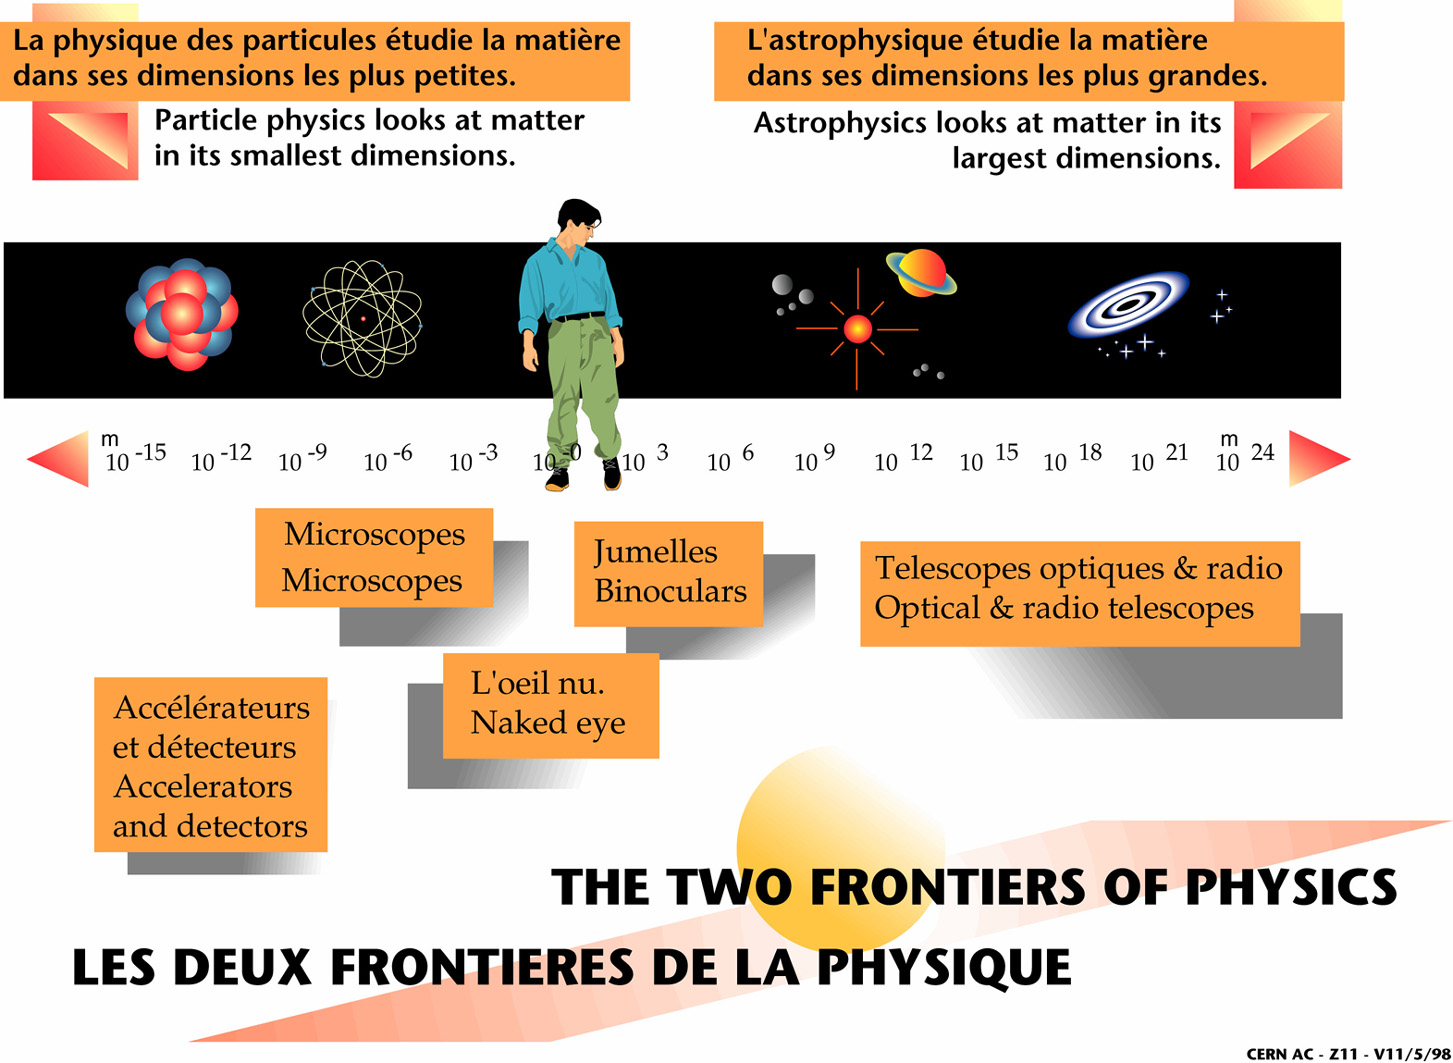
\includegraphics[keepaspectratio,height=14.9cm]{frontiers}
\end{center}

\Tr
\twocolumn[\begin{center}\colorbox{yellow}{Kernfusie laat sterren stralen}\end{center}]
%
\begin{center}
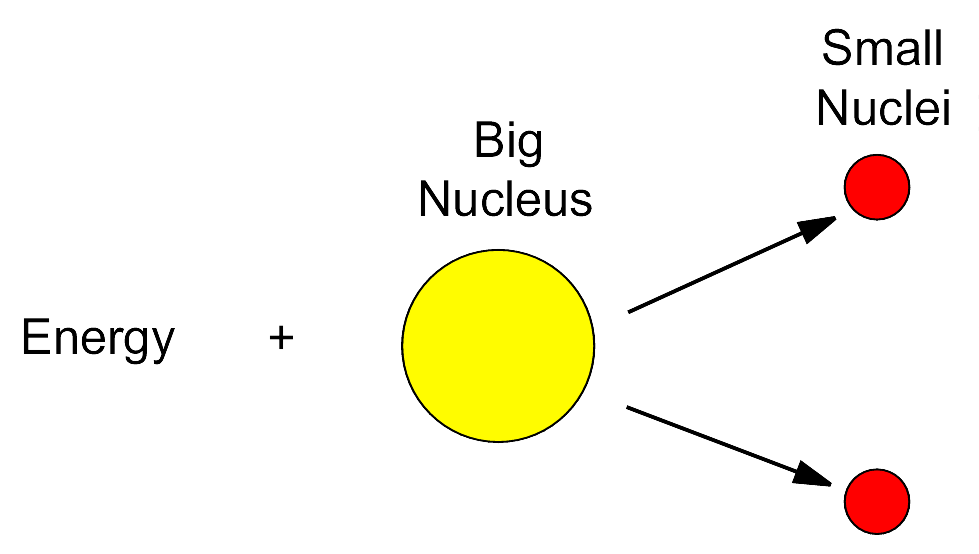
\includegraphics[keepaspectratio,width=10cm]{nuclear-fission}\\[2mm]
{\blue Kernsplitsing}
\end{center}
%
$p+p \rightarrow \Nuc{2}{1}{H}+e^{+}+\nu_{e} \quad \Nuc{2}{1}{H}+p \rightarrow \Nuc{3}{2}{He}+\gamma$ 

\vspace{1cm}

\begin{center}
\colorbox{yellow}{Zwakke kracht produceert neutrinos}\\[2mm]
(Supernovae, AGN, GRBs)
\end{center}
%
\begin{itemize}
\item {\blue Ontstaan van neutronensterren}
\end{itemize}

\newpage
\begin{center}
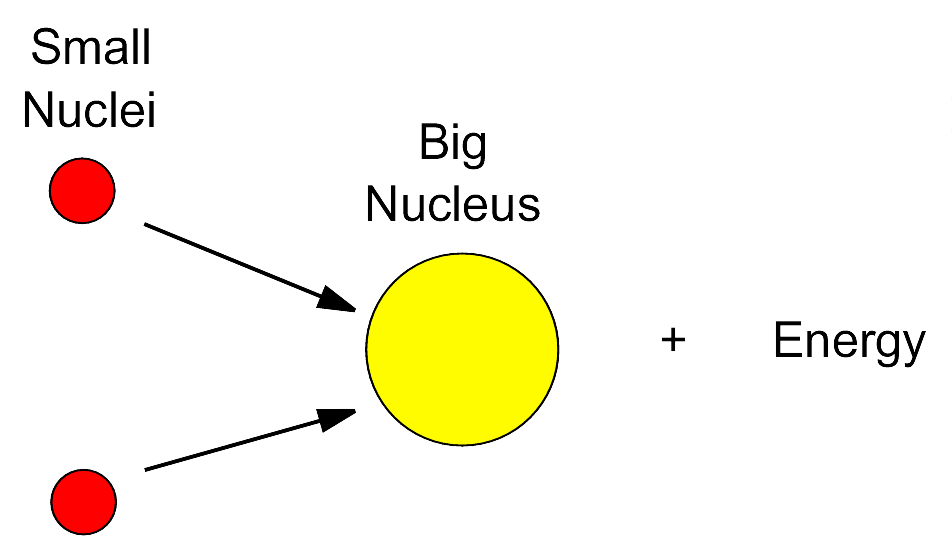
\includegraphics[keepaspectratio,width=10cm]{nuclear-fusion}\\[2mm]
{\blue Kernfusie}
\end{center}
%
$\quad \Nuc{3}{2}{He}+\Nuc{3}{2}{He} \rightarrow \Nuc{4}{2}{He}+p+p$

\vspace{1cm}
\begin{itemize}
\item[] $n \rightarrow p+e^{-}+\bar{\nu}_{e}$
\item[] {\blue $p+e^{-} \rightarrow n+\nu_{e}$}
\item[] $\pi^{-} \rightarrow \mu^{-}+\bar{\nu}_{\mu}$
\item[] $\mu^{-} \rightarrow \nu_{\mu}+e^{-}+\bar{\nu}_{e}$
\end{itemize}

\Tr
\onecolumn
\begin{center}
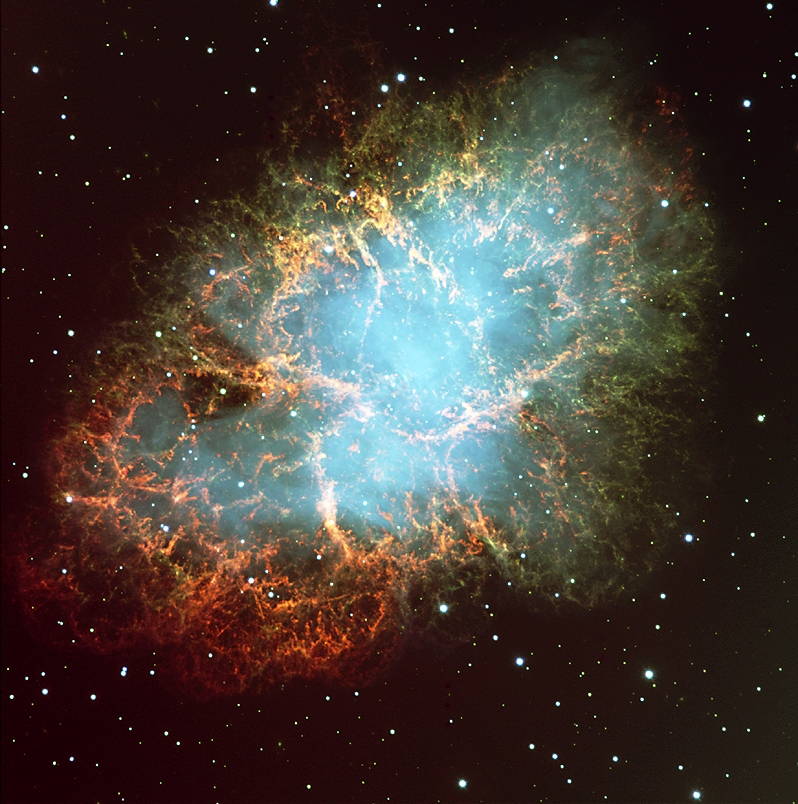
\includegraphics[keepaspectratio,height=15cm]{crab}
\end{center}

\Tr
\begin{center}
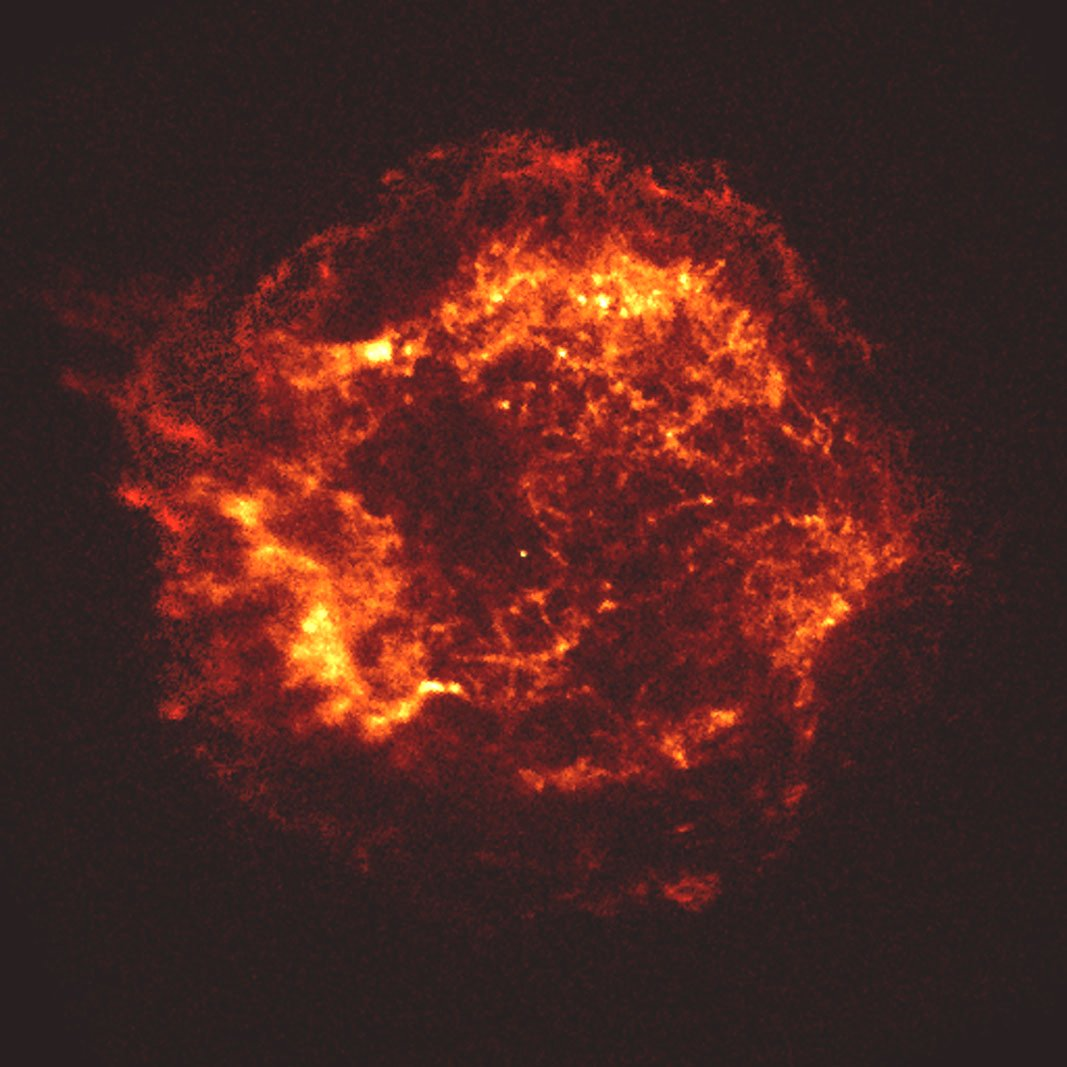
\includegraphics[keepaspectratio,height=15cm]{Cas_A}
\end{center}

\Tr
\twocolumn
\begin{center}
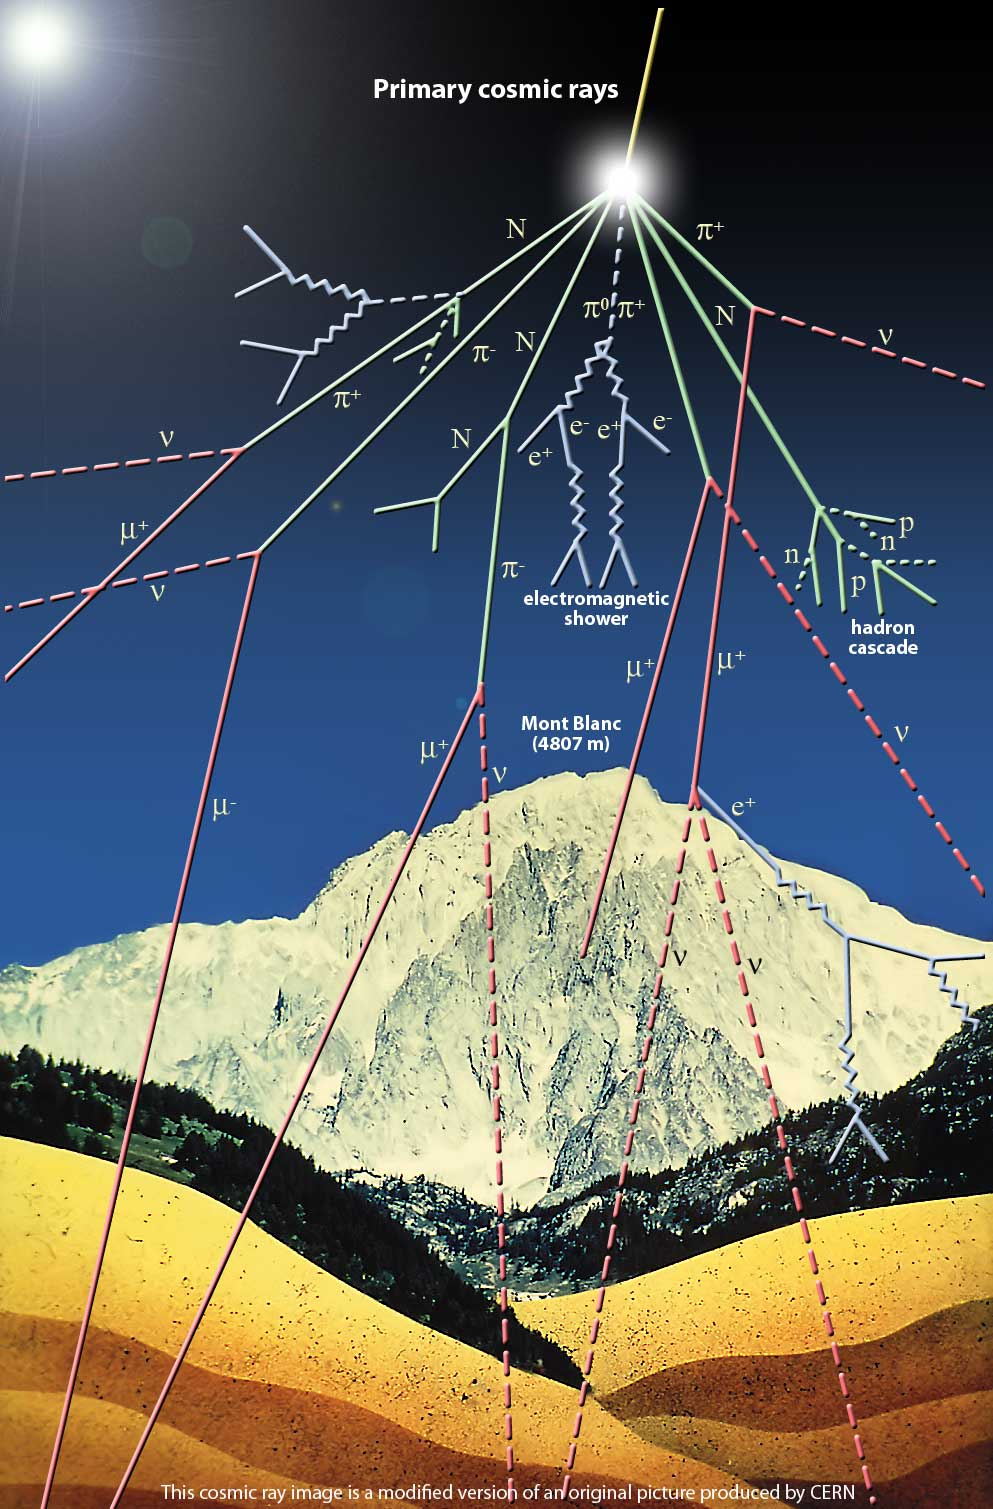
\includegraphics[keepaspectratio,height=15cm]{cosray}
\end{center}

\newpage

\begin{center}
{\blue Spectrum van kosmische straling}\\[5mm]
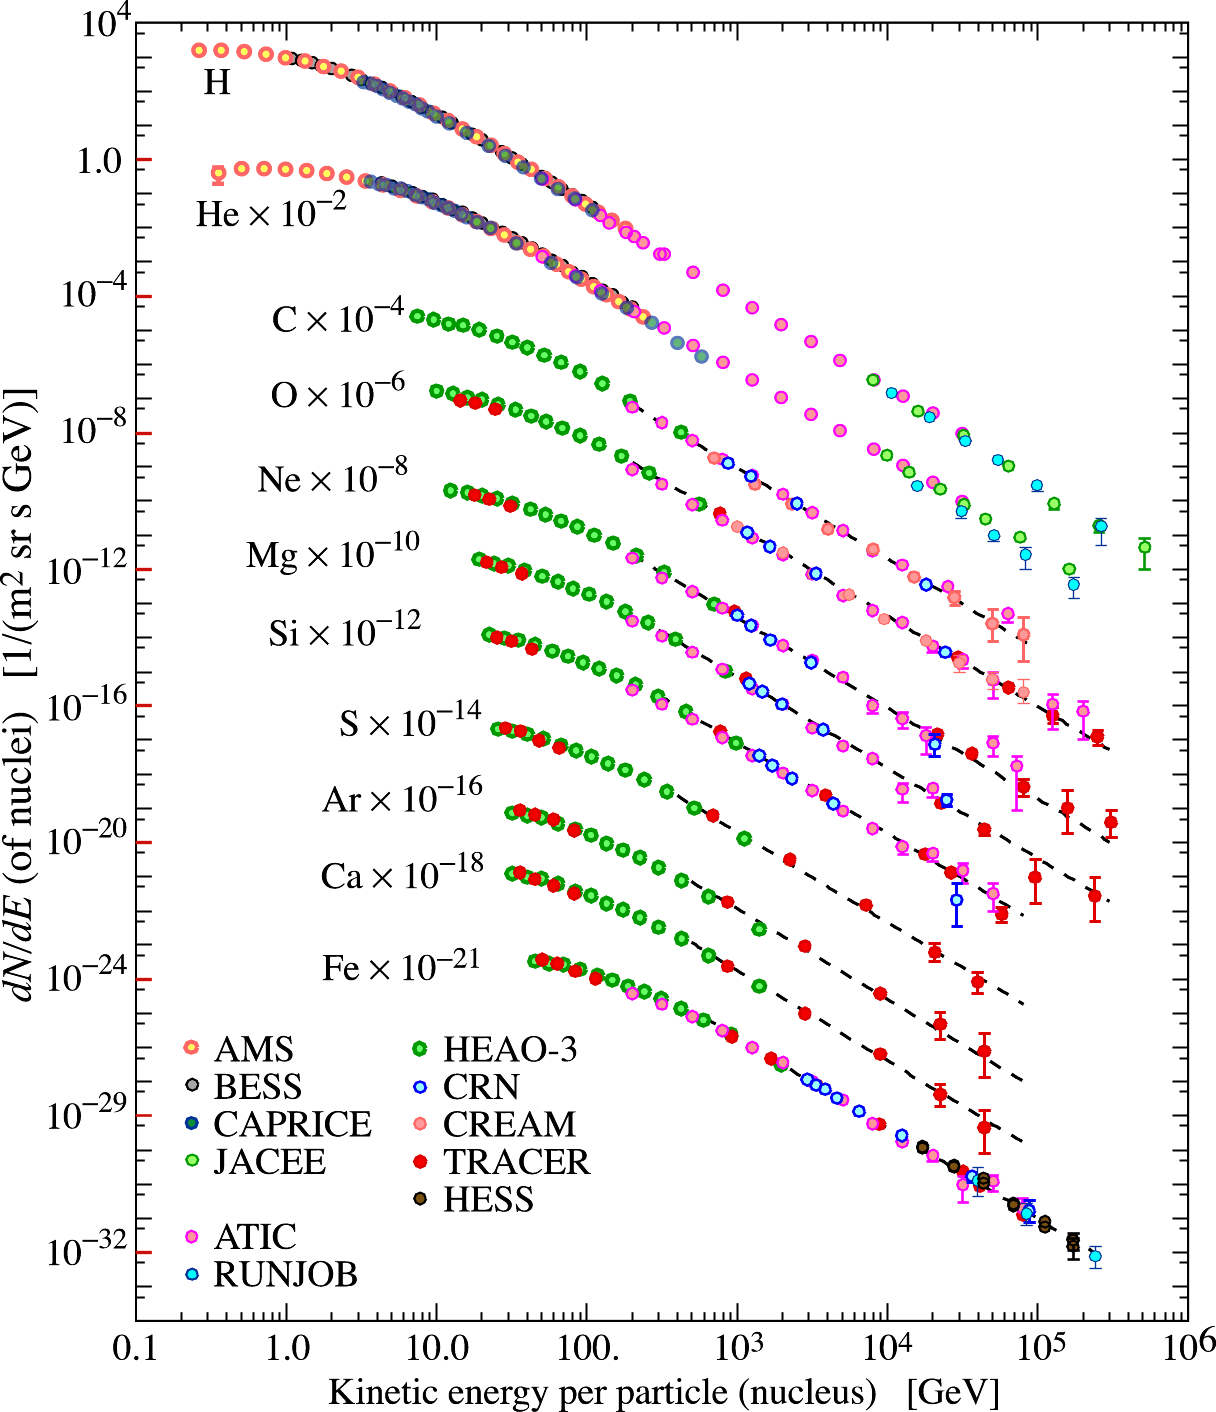
\includegraphics[keepaspectratio,height=14cm]{cr-low-e}
\end{center}

\Tr
\vspace*{1.5cm}
\begin{center}
{\blue $E^{2.6}$ geschaalde flux}\\[5mm]
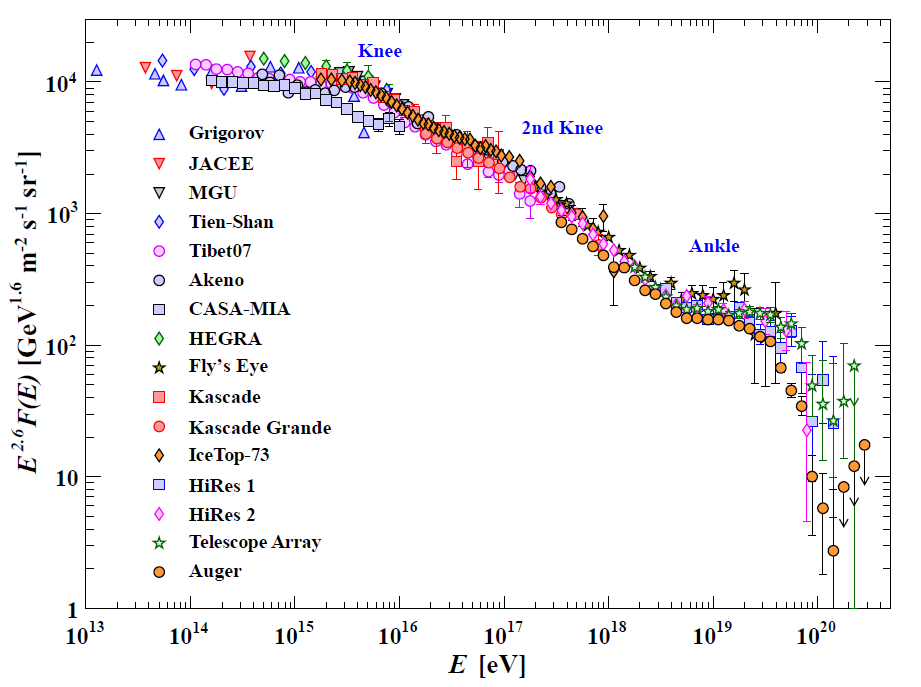
\includegraphics[keepaspectratio,width=13cm]{cr-all-scaled26}
\end{center}

\newpage

\vspace*{3cm}
\begin{itemize}
\item Spectrale structuur (knie, enkel)
\item[] Energetische limieten van kosmische versnellers~?
\item Wat zijn dit voor versnellers~?
\item[] Heftige explosieve fenomenen
\begin{itemize}
\item Supernova's ?
\item Of iets anders ?
\end{itemize}
\end{itemize}

\Tr
\begin{itemize}
\item Supernova schokgolven
\item[] Bewegende lading in mag. veld
\item[] Gyroradius $r=\frac{p}{ZeB} \quad (\vec{p} \perp \vec{B})$
\item[] $\rightarrow
         \left(\frac{p}{1~\rm{eV}}\right)=0.03 \cdot Z\left(\frac{B}{1~\mu\rm{G}}\right)
         \left(\frac{r}{1~\rm{m}}\right)$
\item Versneller van afmeting $R$
\item[] $r > R \rightarrow \text{deeltje~ontsnapt} \rightarrow E_{max}$
\item[] Typisch~: $B \approx \mu\text{G} \quad R \approx 3 \cdot 10^{16}$ m
\item[] $\rightarrow$ Protonen~: $E_{max} \approx 10^{15}$ eV
\item[$\ast$] Bij bepaalde $r \rightarrow {\blue E_{Z}=Z E_{proton}}$
\item[$\ast$] $E>10^{19}~\text{eV} \rightarrow r>R_{melkweg}$
\item[] $\Rightarrow$ Extra-galactische oorsprong
\end{itemize}

\newpage
%
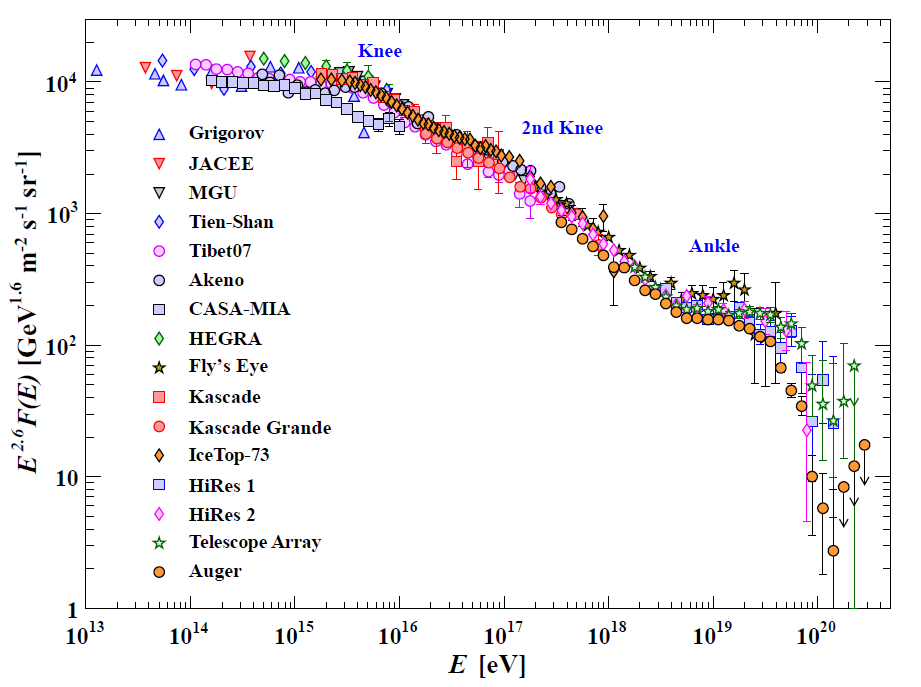
\includegraphics[keepaspectratio,width=13cm]{cr-all-scaled26}
%
\begin{itemize}
\item[] \colorbox{yellow}{Wat veroorzaakt de 'enkel' ?}
\item[] Nog veel krachtigere explosies
\item[] (AGN and GRBs)
\item[] $\rightarrow$ Zwarte gaten
\end{itemize}

\Tr
\begin{center}
{\blue Actieve Melkwegkernen (AGN)}\\[1cm]
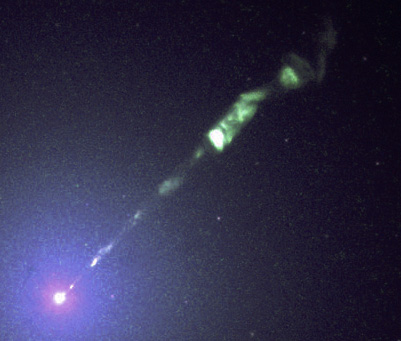
\includegraphics[keepaspectratio,width=13cm]{M87jet}
\end{center}

\newpage

\begin{center}
{\blue Kosmische Gamma Flitsen (GRBs)}\\[1cm]
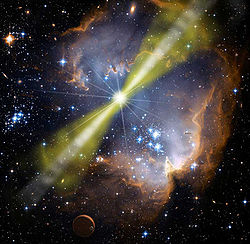
\includegraphics[keepaspectratio,width=6cm]{grb}\\[3mm]
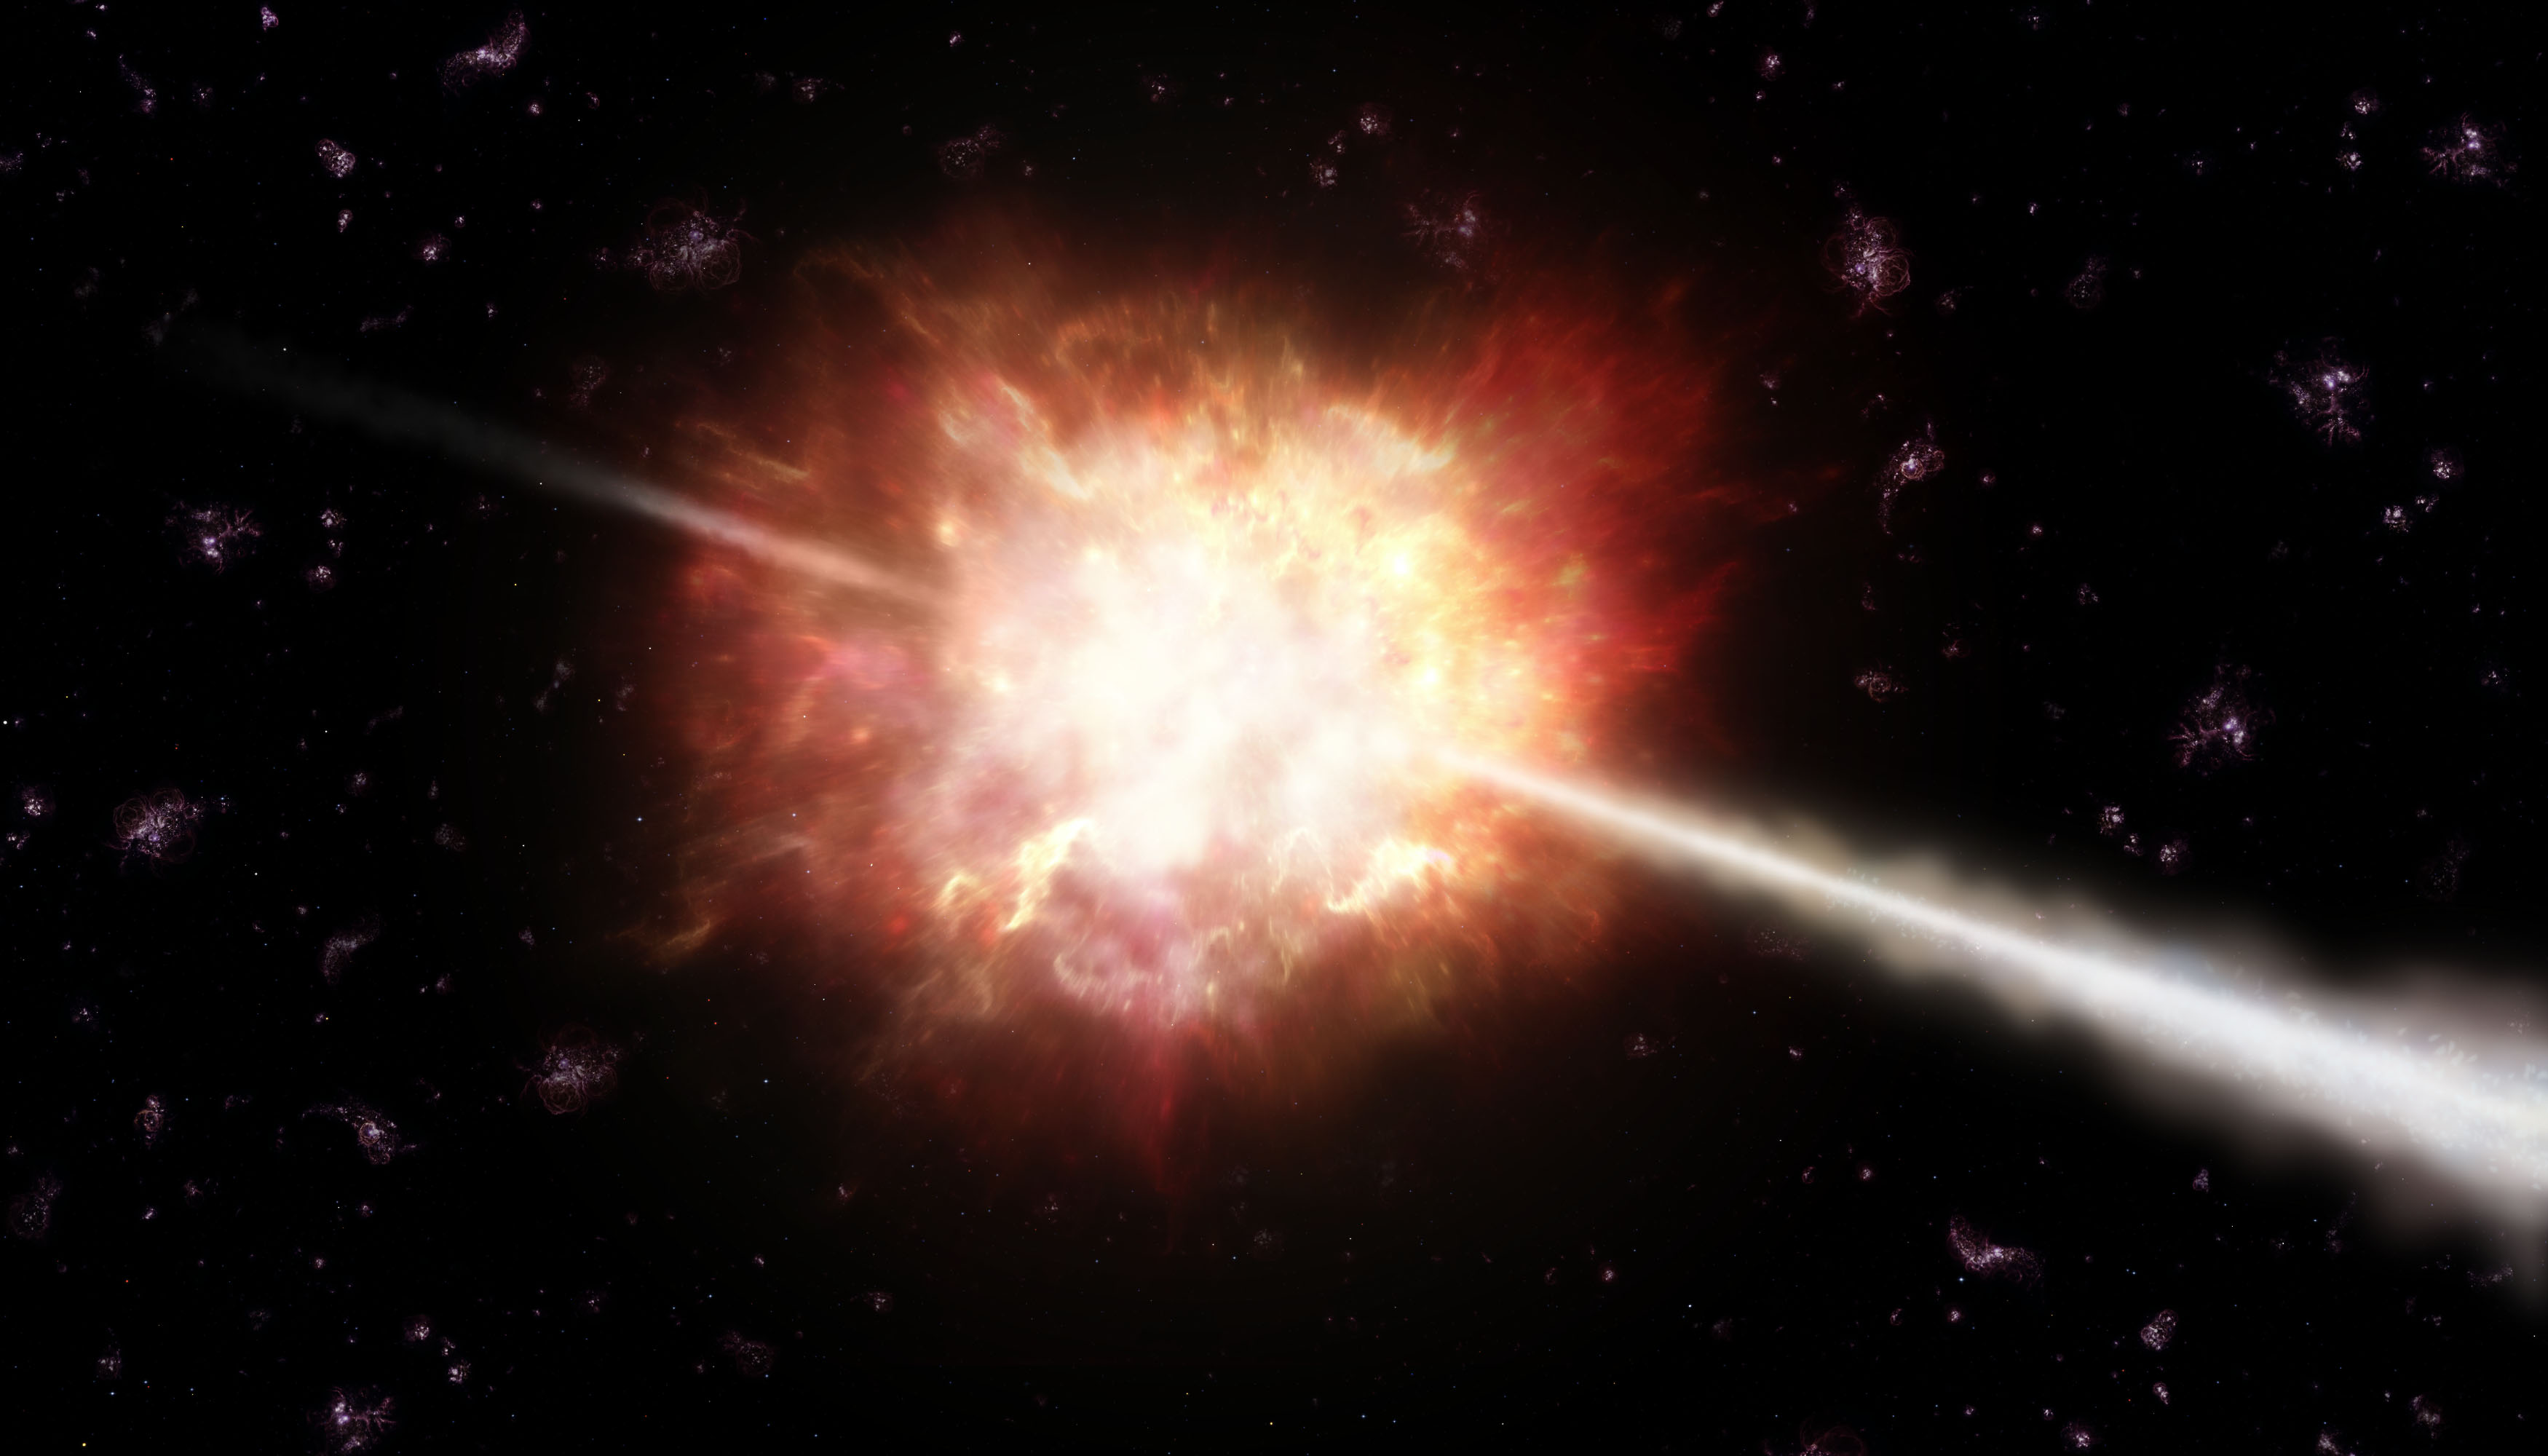
\includegraphics[keepaspectratio,width=12cm]{grb2}
\end{center}

\Tr
\onecolumn
{\blue Waargenomen flitsduur distr. \hspace*{2cm} Mogelijke GRB scenarios}
\begin{center}
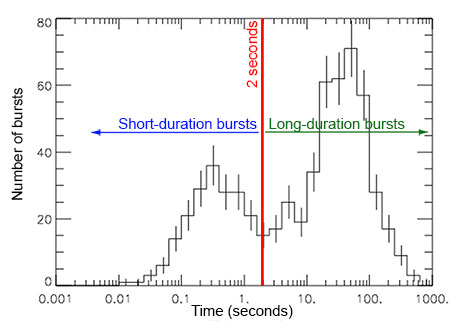
\includegraphics[keepaspectratio,width=10cm]{GRB-T90}
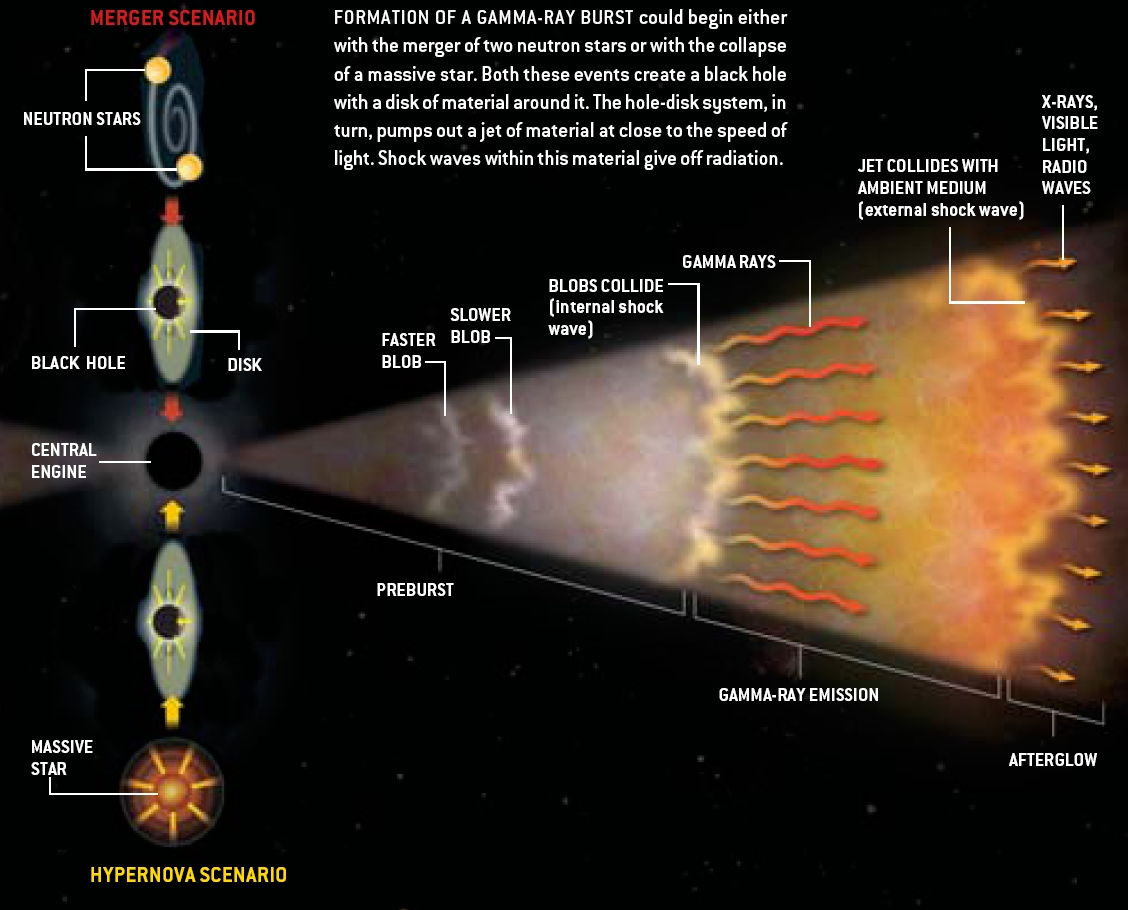
\includegraphics[keepaspectratio,width=16cm]{GRB-phases2}\\[2mm]
{\red Korte GRBs mogelijk ook bronnen van gravitatiegolven} 
\end{center}

\Tr
\twocolumn
\begin{center}
{\blue Algemeen beeld}\\[2mm]
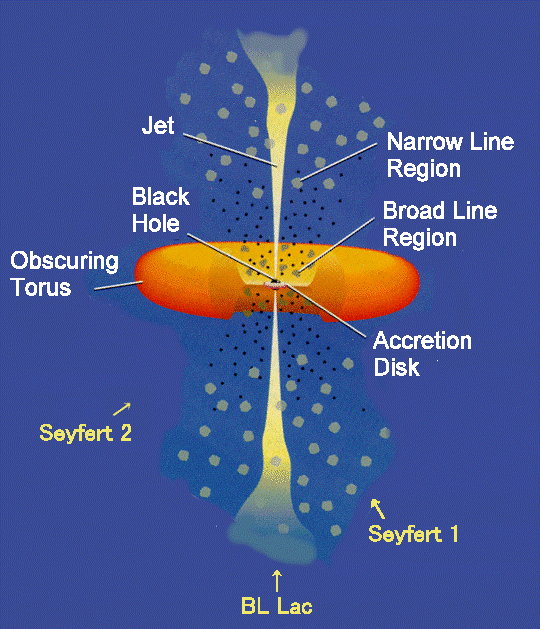
\includegraphics[keepaspectratio,height=12.5cm]{agn-1}\\[5mm]
\colorbox{yellow}{Versnelling in schokgolven}
\end{center}

\newpage

\begin{center}
{\blue Fysische processen}\\[5mm]
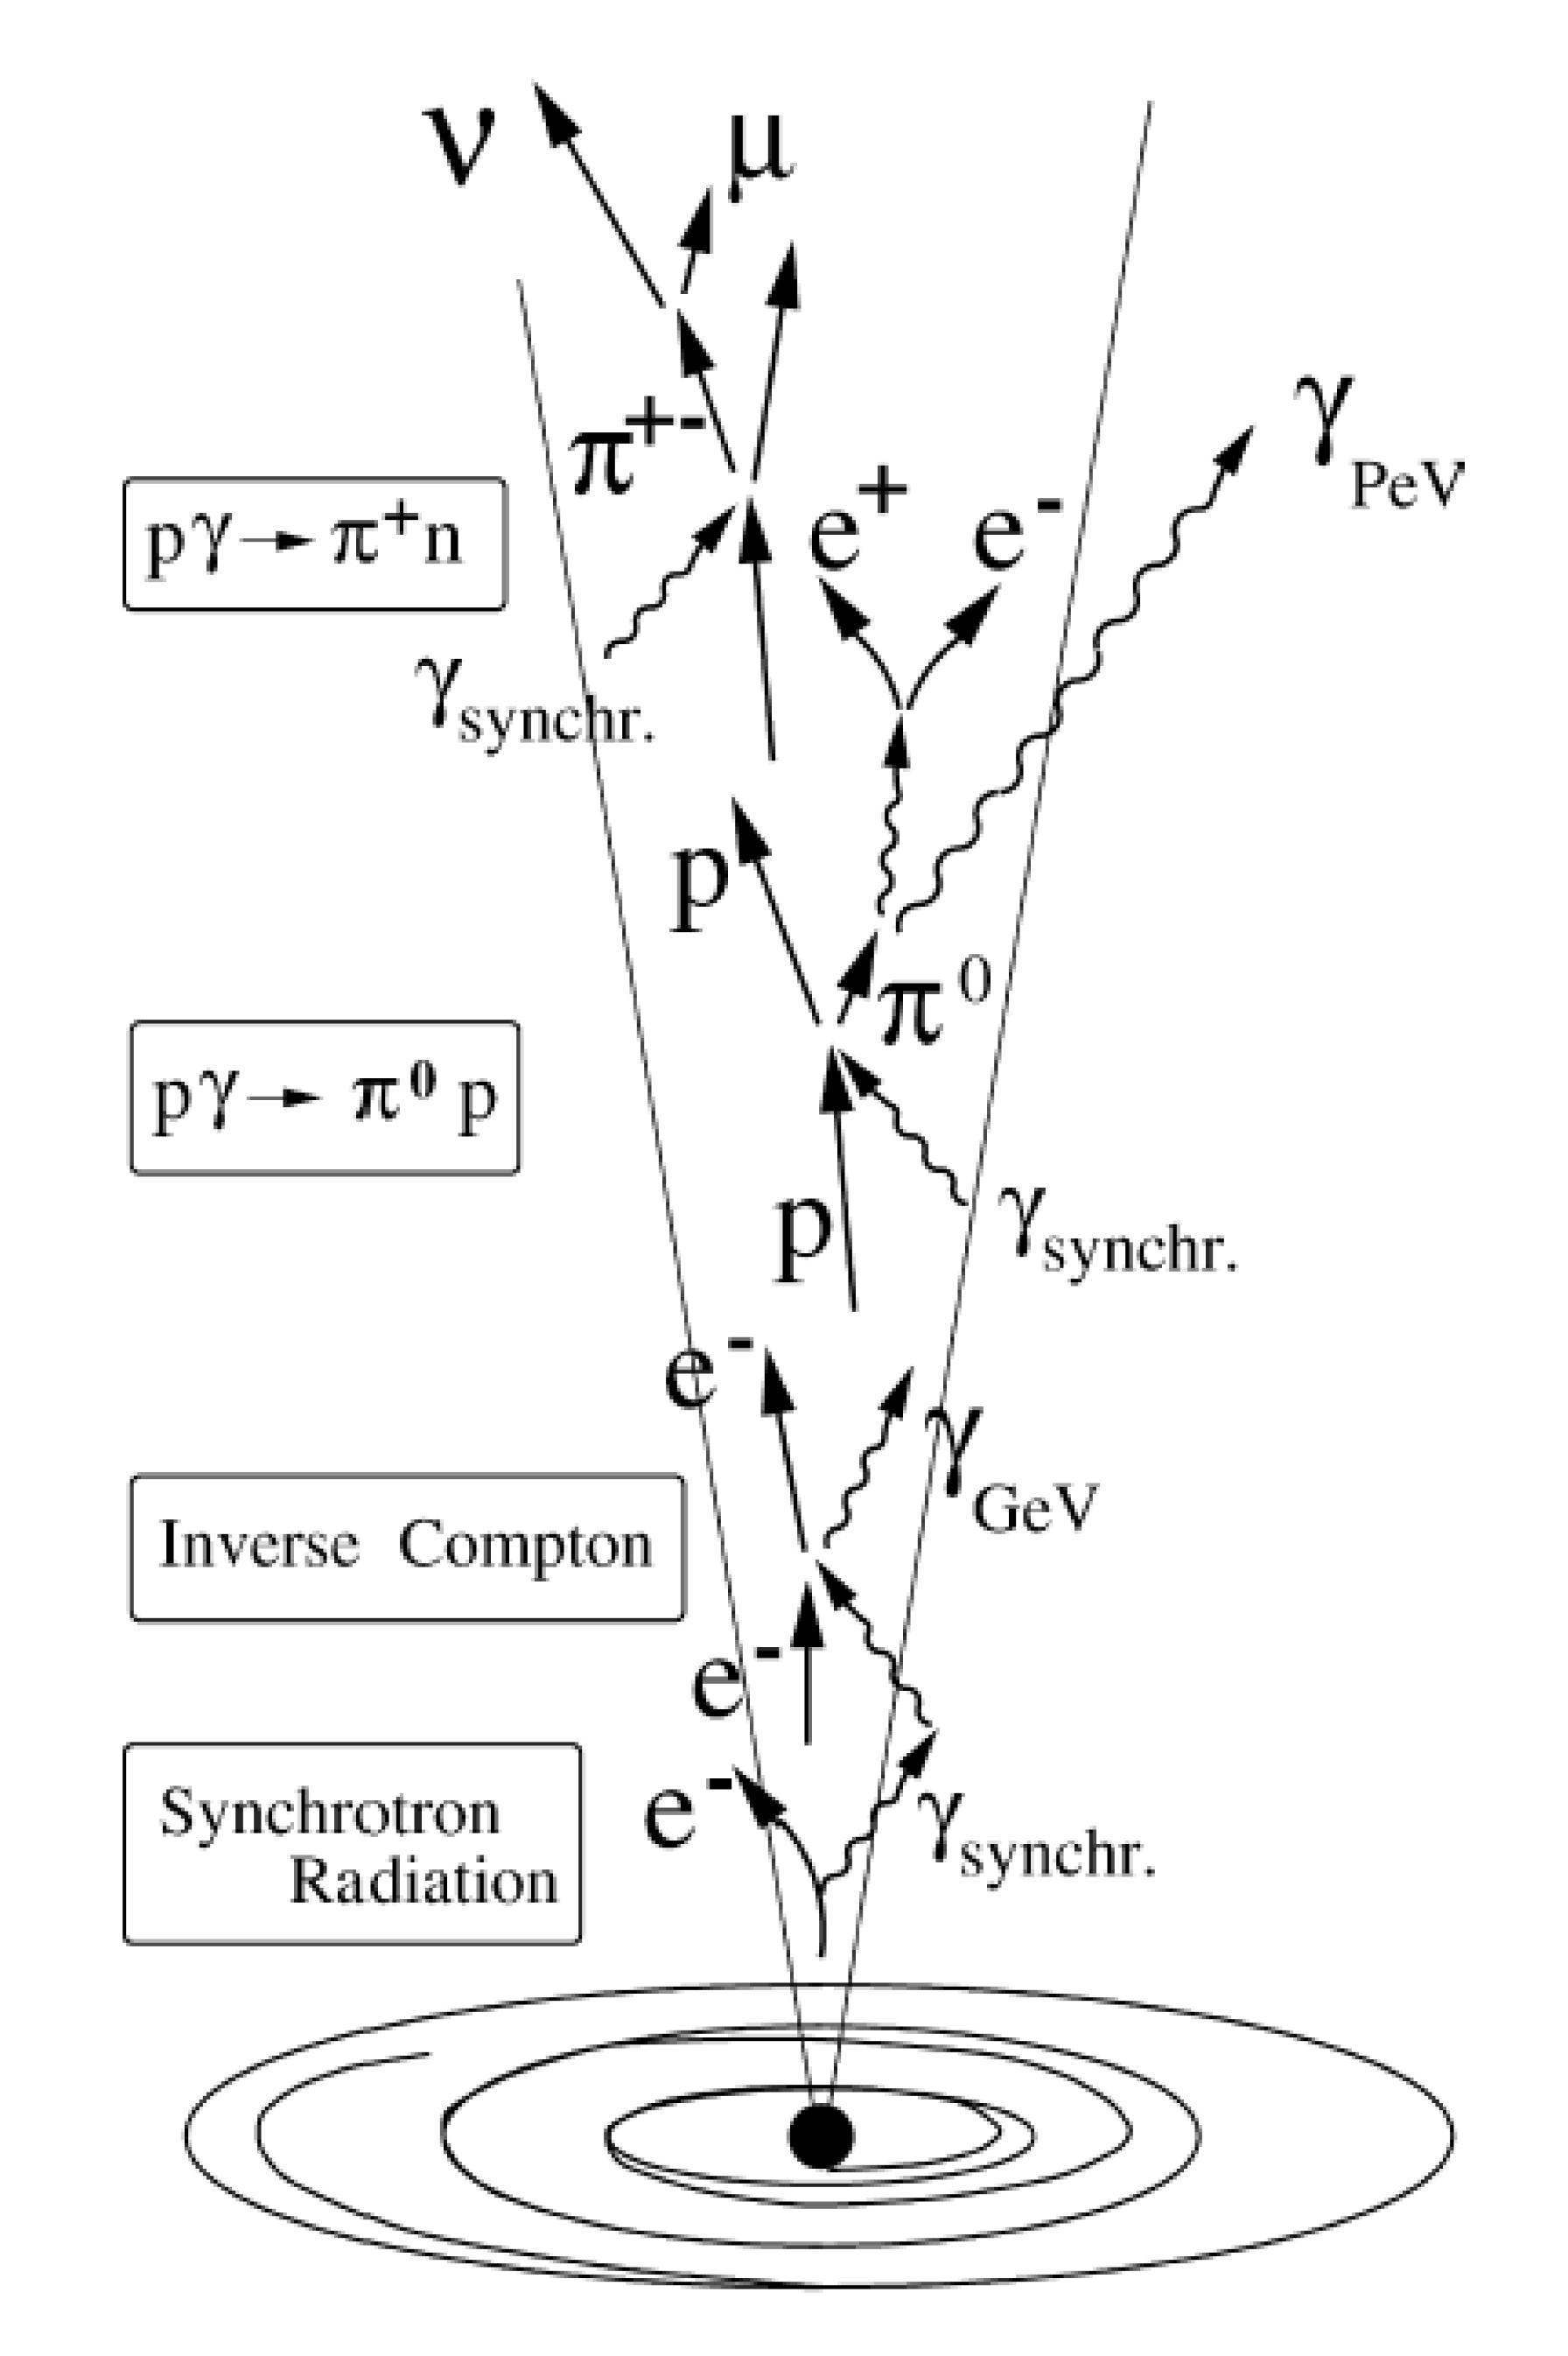
\includegraphics[keepaspectratio,height=12.3cm]{jet}\\[5mm]
\colorbox{yellow}{Hoog-energetische fotonen en neutrinos}
\end{center}
